\input{../style/preamble}
\input{../latex-math/basic-math}
\input{../latex-math/basic-ml}
\input{../latex-math/ml-nn}

% The course's typewriter font (laett) has no bold shape; map bold typewriter to regular.
\AtBeginDocument{{\ttfamily\selectfont}\DeclareFontShape{T1}{laett}{bx}{n}{<->ssub*laett/m/n}{}\DeclareFontShape{T1}{laett}{m}{bx}{<->ssub*laett/m/n}{}}
\newcommand{\citebutton}[2]{\beamergotobutton{\href{#2}{#1}}}

\newcommand{\titlefigure}{figure/vit-summary.png}
\newcommand{\learninggoals}{
  \item Vision Transformers: images as patch sequences, inductive bias, transfer learning; Swin's shifted windows
  \item DETR and MaskFormer: detection and segmentation with a Transformer decoder and set-based loss
  \item Knowledge distillation for vision models
  \item Vision language models, contrastive learning, CLIP, BLIP and OWL-ViT
  \item Video Transformers: ViViT and TimeSformer
}

\title{Advanced Artificial Intelligence and Machine Learning}
\date{}

\begin{document}

\lecturechapter{Transformers Outside NLP}
\lecture{Advanced AI \& ML}

%%%%%%%%%%%%%%%%%%%%%%%%%%%%%%%%%%%%%%%%%%%%%%%%%%%%%%%%%%%%%%%%%%
\section{Vision Transformers for Image Classification}
% Source: HF CV course, unit3/vision-transformers/vision-transformers-for-image-classification
%%%%%%%%%%%%%%%%%%%%%%%%%%%%%%%%%%%%%%%%%%%%%%%%%%%%%%%%%%%%%%%%%%

\begin{frame}{Vision Transformer (ViT)}
\begin{itemize}
  \item As the Transformer architecture scaled well in NLP, the same architecture was applied to images by creating small patches of the image and treating them as tokens: the \textbf{Vision Transformer (ViT)}.
  \item Images are reorganized as 2D grids of patches; the model is trained on those patches.
\end{itemize}
\begin{figure}
  \centering
  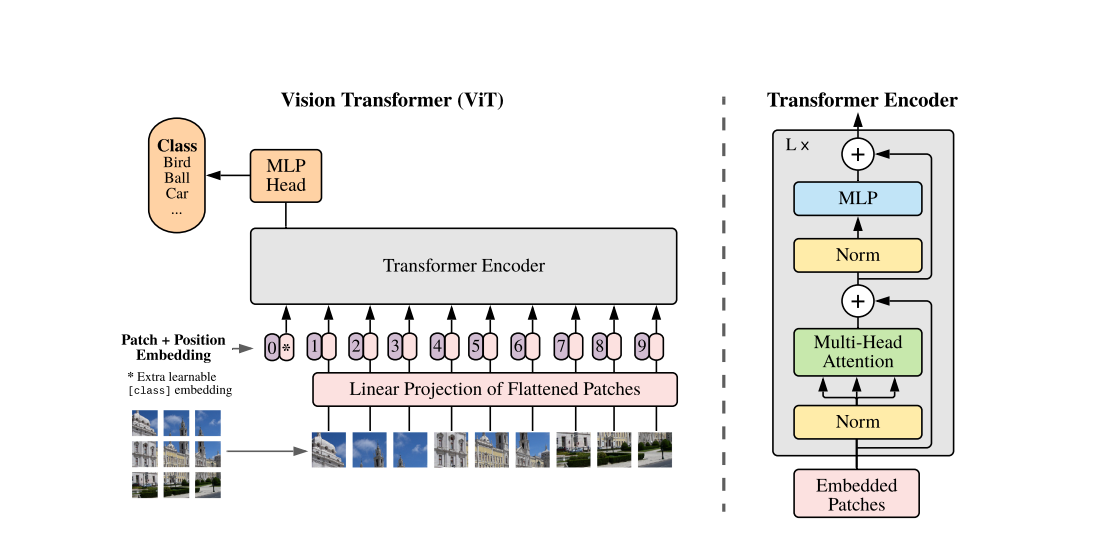
\includegraphics[width=0.62\textwidth]{figure/vit-summary.png}\\
  \citebutton{Source: Dosovitskiy et al., 2020}{https://arxiv.org/abs/2010.11929}
\end{figure}
\end{frame}

\begin{frame}{CNNs vs.\ Vision Transformers: Inductive Bias}
\small% fit16:9
\begin{itemize}
  \item \textbf{Inductive bias}: the set of assumptions a learning algorithm uses to make predictions --- a shortcut that helps a model make educated guesses based on what it has seen so far.
  \item Two inductive biases of CNNs:
  \begin{itemize}
    \item \textbf{Translational equivariance}: an object can appear anywhere in the image, and CNNs can detect its features.
    \item \textbf{Locality}: pixels interact mainly with their surrounding pixels to form features.
  \end{itemize}
  \item ViT does not have these assumptions. That is why, up to a certain dataset size, CNNs are actually better than ViT.
  \item But: being (mostly) different types of linear functions, the Transformer makes ViT highly scalable --- which lets ViT overcome the missing inductive biases with massive amounts of data.
\end{itemize}
\end{frame}

\begin{frame}{Transfer Learning \& Fine-Tuning}
\begin{itemize}
  \item Training a ViT on millions of images is not feasible for everyone. Instead, use openly available pre-trained weights (e.g.\ the Hugging Face Hub).
  \item \textbf{Transfer learning}: leverage the features a ViT learned on a very large dataset and apply them to our (possibly small) dataset.
  \begin{itemize}
    \item By freezing most of the weights, we train only certain layers: good performance with less training time and low GPU consumption.
  \end{itemize}
  \item \textbf{Fine-tuning}: if our domain differs from the pre-training data, update the weights of the entire pre-trained model, with a lower learning rate.
  \item In most scenarios, transfer learning is ample for Vision Transformers.
  \item Both work for \textbf{multi-class} (one label per image) and \textbf{multi-label} (several labels per image) classification.
\end{itemize}
\end{frame}

%%%%%%%%%%%%%%%%%%%%%%%%%%%%%%%%%%%%%%%%%%%%%%%%%%%%%%%%%%%%%%%%%%
\section{Swin Transformer}
% Source: HF CV course, unit3/vision-transformers/swin-transformer
%%%%%%%%%%%%%%%%%%%%%%%%%%%%%%%%%%%%%%%%%%%%%%%%%%%%%%%%%%%%%%%%%%

\begin{frame}{Swin Transformer}
\begin{itemize}
  \item Introduced in 2021 \citebutton{Liu et al., 2021}{https://arxiv.org/abs/2103.14030}: optimizes for latency and performance using a \textbf{shifted window} (as opposed to sliding window) approach, which reduces the number of operations required.
  \item Swin is a \textbf{hierarchical backbone} for computer vision, e.g.\ for image classification.
  \begin{itemize}
    \item A \textit{backbone} is the part of a network that does feature extraction; additional layers can be added on top for a variety of vision tasks.
    \item \textit{Hierarchical} backbones have tiered structures, sometimes with varying resolutions --- in contrast to the non-hierarchical \textit{plain} backbone of e.g.\ ViTDet.
  \end{itemize}
\end{itemize}
\end{frame}

\begin{frame}{Shifted Windows}
\begin{itemize}
  \item In the original ViT, attention is done between each patch and all other patches --- computationally intensive.
  \item Swin reduces ViT's quadratic complexity to \textbf{linear} complexity (w.r.t.\ image size): similar to a CNN, patches only attend to other patches in the \textbf{same window}, and are then gradually merged with neighboring patches. This is what makes Swin hierarchical.
\end{itemize}
\begin{figure}
  \centering
  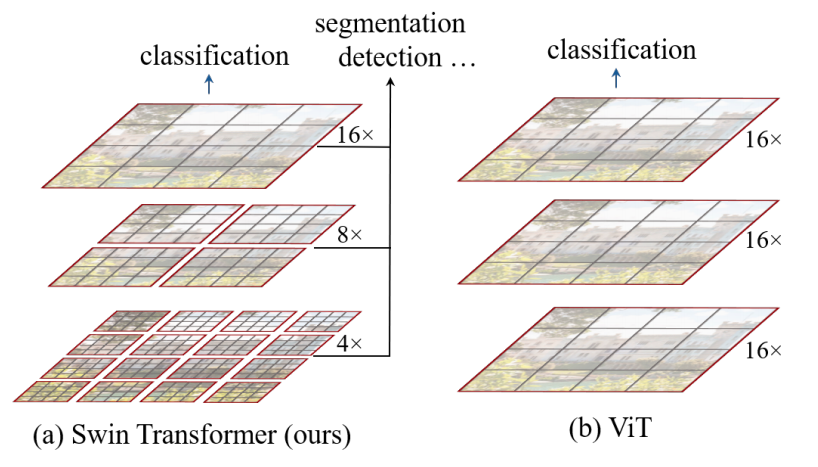
\includegraphics[width=0.42\textwidth]{figure/swin-vs-vit.png}\\
  \citebutton{Source: Liu et al., 2021}{https://arxiv.org/abs/2103.14030}
\end{figure}
\end{frame}

\begin{frame}{Swin: Advantages and Successors}
\begin{itemize}
  \item \textbf{Computational efficiency}: Swin is more performant than completely patch-based approaches like ViT.
  \item \textbf{Large datasets}: as training size goes up, Swin outperforms CNNs; the large number of parameters enables increased capacity for learning more complex representations.
  \item \textbf{Swin Transformer V2} \citebutton{Liu et al., 2022}{https://arxiv.org/abs/2111.09883}: one of the first 3B-parameter vision models, trainable with high-resolution images. It stabilizes training, transfers models pre-trained on low-resolution images to high-resolution tasks, and uses SimMIM, a self-supervised approach that reduces the number of labeled images required.
  \item \textbf{Image restoration}: SwinIR turns low-resolution into high-resolution images; Swin2SR improves on it using Swin V2.
\end{itemize}
\end{frame}

\begin{frame}{Swin Implementation: The Model}
\small% fit16:9
Key parts of the original PyTorch implementation:
\begin{enumerate}
  \item \textbf{Parameters}, among others: \texttt{window\_size} (size of the windows for local self-attention), \texttt{ape} (add absolute position embeddings?).
  \item \textbf{Patch embedding}: similar to ViT, the image is split into non-overlapping patches, linearly embedded using a \texttt{Conv2D}.
  \item \textbf{Positional embeddings} (optional, \texttt{ape}): added to the patch embeddings to help the model use positional information about each patch.
  \item \textbf{Stochastic depth decay}: regularization by skipping layers during training --- the deeper the layer, the higher the chance it is skipped.
  \item \textbf{Layers}: multiple \texttt{BasicLayer}s of \texttt{SwinTransformerBlock}s, each downsampling the feature map via \texttt{PatchMerging}. Feature dimensionality and resolution change across layers.
  \item \textbf{Classification head}: as in ViT, an MLP head.
\end{enumerate}
\end{frame}

\begin{frame}{Swin Implementation: The Block}
\textbf{Components:} LayerNorm $\to$ \textbf{window attention} (self-attention within local windows) $\to$ drop path (stochastic depth) $\to$ LayerNorm $\to$ MLP; an \textbf{attention mask} controls which elements in the windowed input may attend to each other.

\vspace{0.2cm}
\textbf{Forward pass, four steps:}
\begin{enumerate}
  \item \textbf{Cyclic shift}: the feature map is partitioned into windows, and the partitions are cyclically shifted (e.g.\ \texttt{A, B, C, D} shifted right by one becomes \texttt{D, A, B, C}). This lets the model capture relationships between adjacent windows.
  \item \textbf{Windowed attention}: window-based multi-head self-attention (W-MSA).
  \item \textbf{Merge patches} via \texttt{PatchMerging}.
  \item \textbf{Reverse cyclic shift}: window partitioning and shift are undone, so the feature map retains its original form.
\end{enumerate}
\end{frame}

\begin{frame}{Window Attention and Patch Merging}
\begin{itemize}
  \item \textbf{Window attention}: window-based multi-head self-attention (W-MSA) with relative position bias; used for both shifted and non-shifted windows.
  \item \textbf{Patch merging}: downsampling. Reduces the spatial dimensions of the feature map, similar to pooling in CNNs --- building hierarchical feature representations by progressively increasing the receptive field and reducing the spatial resolution.
\end{itemize}
\end{frame}

%%%%%%%%%%%%%%%%%%%%%%%%%%%%%%%%%%%%%%%%%%%%%%%%%%%%%%%%%%%%%%%%%%
\section{DEtection TRansformer (DETR)}
% Source: HF CV course, unit3/vision-transformers/detr
%%%%%%%%%%%%%%%%%%%%%%%%%%%%%%%%%%%%%%%%%%%%%%%%%%%%%%%%%%%%%%%%%%

\begin{frame}{Object Detection with DETR}
\begin{itemize}
  \item \textbf{Object detection}: detect objects in an image. Input: e.g.\ an image of a road. Output: e.g.\ \texttt{[('car',X1,Y1,W1,H1), ('pedestrian',X2,Y2,W2,H2)]} --- class, plus the $x,y$ coordinates, width and height of each bounding box.
  \item Traditional detectors like YOLO use hand-crafted features such as \textbf{anchor box priors} (initial guesses of object locations and shapes), and post-processing steps to remove overlapping boxes, which need carefully selected filtering heuristics.
  \item \textbf{DETR} \citebutton{Carion et al., 2020}{https://arxiv.org/abs/2005.12872} simplifies the detector: an encoder-decoder Transformer after the feature-extraction backbone \textbf{directly predicts bounding boxes in parallel}, requiring minimal post-processing.
\end{itemize}
\end{frame}

\begin{frame}{DETR: Architecture}
\begin{figure}
  \centering
  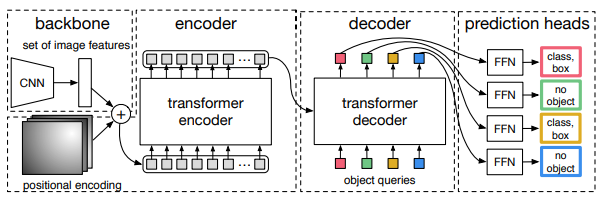
\includegraphics[width=0.61\textwidth]{figure/detr-architecture.png}\\
  \citebutton{Source: Carion et al., 2020}{https://arxiv.org/abs/2005.12872}
\end{figure}
\begin{itemize}
  \item A CNN backbone; its output is fed into a Transformer encoder, resulting in $N$ embeddings.
  \item The decoder uses learned positional embeddings (\textbf{object queries}) and the encoder output, generating another $N$ embeddings.
  \item Each of the $N$ embeddings goes through feed-forward layers predicting the bounding box (coordinates, width, height) and the object class --- or that there is no object.
\end{itemize}
\end{frame}

\begin{frame}{DETR: Encoder-Decoder}
\begin{itemize}
  \item The encoder expects a sequence, so the backbone's feature map of size \texttt{[dimension, height, width]} is downsized and flattened to \texttt{[dimension, less than height $\times$ width]}.
\end{itemize}
\begin{figure}
  \centering
  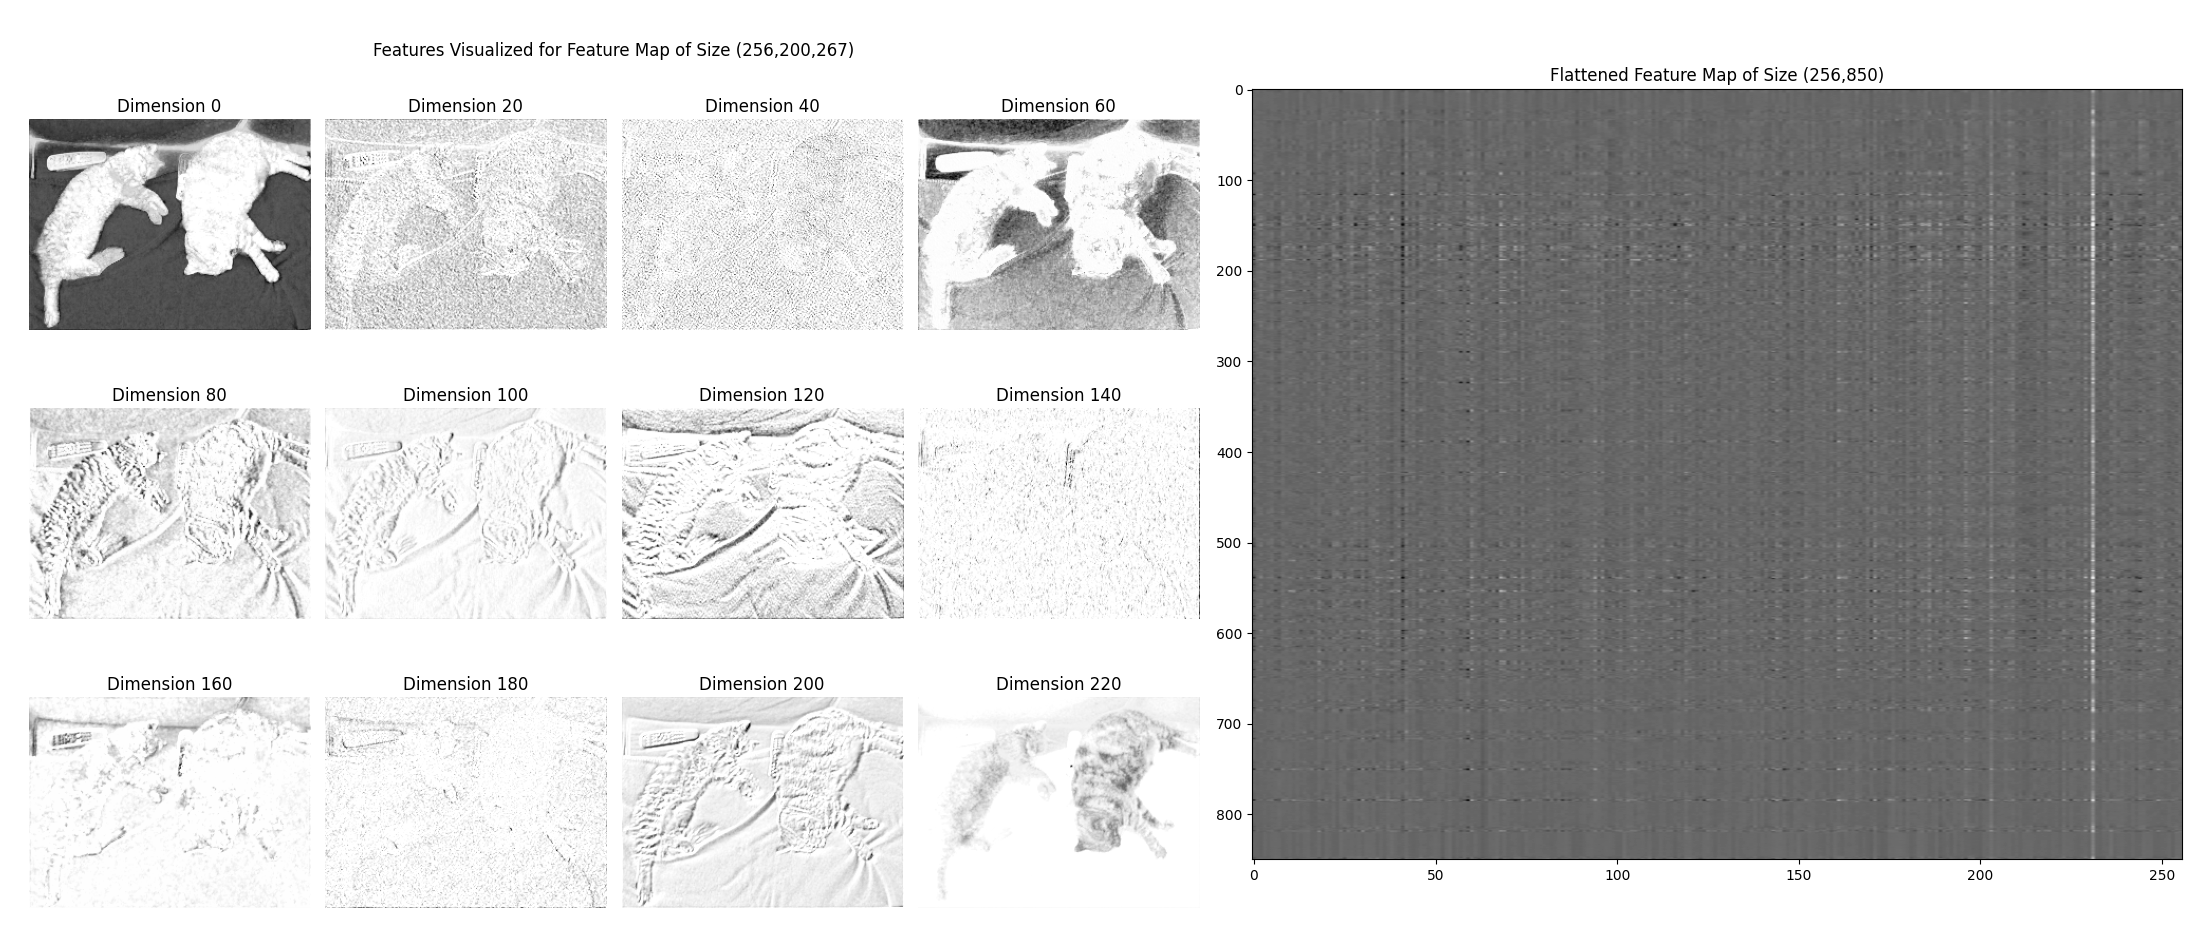
\includegraphics[width=0.7\textwidth]{figure/detr-feature-maps.png}
\end{figure}
{\footnotesize Left: 12 of 256 feature-map dimensions; each extracts some features of the cat image (some focus on the cat's patterns, some on the bed sheets). Right: keeping 256 dimensions, width and height are flattened into size 850.}
\end{frame}

\begin{frame}{DETR: Positional Embeddings}
\begin{itemize}
  \item Transformers are permutation invariant, so positional embeddings are added in both encoder and decoder to remind the model where in the image an embedding comes from.
  \item \textbf{Encoder: fixed} positional encodings, as in the original Transformer --- sinusoidal functions of varying frequencies at different feature dimensions. A sense of position without learned parameters.
  \item \textbf{Decoder: learned} positional encodings (the object queries) --- each position has its own encoding, learned during training.
\end{itemize}
\end{frame}

\begin{frame}{DETR: Set-Based Global Loss}
\footnotesize% fit16:9

\begin{itemize}
  \item YOLO's loss: bounding box, objectness (probability that an object exists in a region of interest) and class loss, computed over a fixed number of boxes per grid cell.
  \item DETR generates unique bounding boxes in a \textbf{permutation-invariant} manner: the order of the detections does not matter, and the boxes must differ from each other. So predictions must be \textbf{matched} to the ground truth before they can be scored.
  \item \textbf{Bipartite matching}: a one-to-one matching between ground-truth and predicted boxes, pairing those with the highest similarity in box and class.
  \begin{itemize}
    \item The closest prediction is matched with the corresponding ground truth, so boxes and classes are adjusted properly in the loss.
    \item Without matching, a correct prediction that is not in the same order as the ground truth would be marked incorrect.
  \end{itemize}
\end{itemize}
\end{frame}

\begin{frame}{Evolution of DETR: Deformable DETR}
\small% fit16:9
Two main problems of DETR: long, slow convergence, and suboptimal detection of small objects.
\begin{itemize}
  \item \textbf{Deformable attention} (fixes slow convergence): global attention is inefficient and heavily limits image resolution. Instead, the model attends only to a fixed number of \textit{sampling points} around each \textit{reference point}; the reference points are learned from the input.
  \begin{itemize}
    \item E.g.\ in an image of a dog, a reference point may be at the dog's center, with sampling points near the ears, mouth, tail.
  \end{itemize}
  \item \textbf{Multi-scale deformable attention} (fixes small objects): as in YOLOv3, multi-scale feature maps. Different layers of deformable attention give different resolutions; connecting some encoder layers' outputs to the decoder lets the model detect objects of many sizes.
\end{itemize}
\end{frame}

\begin{frame}{Evolution of DETR: Conditional DETR}
\begin{itemize}
  \item Also targets slow convergence: over 6.7$\times$ faster. The object queries turn out to be general, not specific to the input image; \textbf{conditional cross-attention} lets the queries better localize the regions for box regression.
  \item Content query $c_q$ (decoder self-attention output) and spatial query $p_q$: DETR adds them, Conditional DETR \textbf{concatenates} them --- $c_q$ focuses on the object's content, $p_q$ on the box region.
\end{itemize}
\begin{figure}
  \centering
  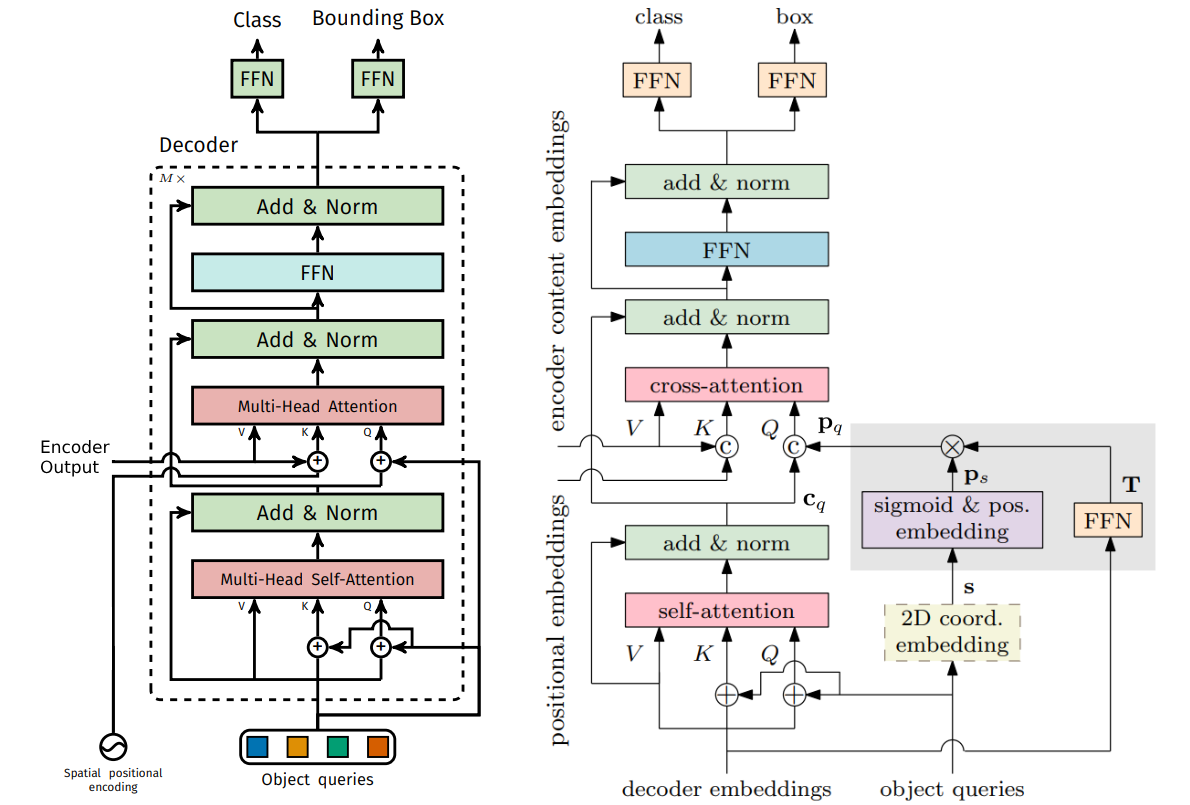
\includegraphics[width=0.23\textwidth]{figure/detr-decoder-layer.png}\\
  {\footnotesize Left: DETR decoder layer. Right: Conditional DETR decoder layer.} \citebutton{Source: Meng et al., 2021}{https://arxiv.org/abs/2108.06152}
\end{figure}
\end{frame}

\begin{frame}[fragile]{DETR: PyTorch Implementation}
\vspace{-0.3cm}
\tiny
\begin{verbatim}
class DETR(nn.Module):
    def __init__(self, num_classes, hidden_dim, nheads, num_encoder_layers, num_decoder_layers):
        super().__init__()
        self.backbone = nn.Sequential(*list(resnet50(pretrained=True).children())[:-2])
        self.conv = nn.Conv2d(2048, hidden_dim, 1)
        self.transformer = nn.Transformer(hidden_dim, nheads, num_encoder_layers, num_decoder_layers)
        self.linear_class = nn.Linear(hidden_dim, num_classes + 1)
        self.linear_bbox = nn.Linear(hidden_dim, 4)
        self.query_pos = nn.Parameter(torch.rand(100, hidden_dim))
        self.row_embed = nn.Parameter(torch.rand(50, hidden_dim // 2))
        self.col_embed = nn.Parameter(torch.rand(50, hidden_dim // 2))

    def forward(self, inputs):
        x = self.backbone(inputs)
        h = self.conv(x)
        H, W = h.shape[-2:]
        pos = torch.cat([self.col_embed[:W].unsqueeze(0).repeat(H, 1, 1),
                         self.row_embed[:H].unsqueeze(1).repeat(1, W, 1)],
                        dim=-1).flatten(0, 1).unsqueeze(1)
        h = self.transformer(pos + h.flatten(2).permute(2, 0, 1), self.query_pos.unsqueeze(1))
        return self.linear_class(h), self.linear_bbox(h).sigmoid()
\end{verbatim}
\normalsize
\vspace{-0.3cm}
{\footnotesize The implementation from the original paper \citebutton{Carion et al., 2020}{https://arxiv.org/abs/2005.12872}, as shown in the HF course.}
\end{frame}

\begin{frame}{DETR: The \texttt{forward} Function, Line by Line}
\footnotesize% fit16:9

\begin{itemize}
  \item \textbf{Backbone}: the image goes through a ResNet backbone, then a convolution reducing the dimension to \texttt{hidden\_dim}.
  \item \textbf{Positional embeddings}: the paper uses fixed (encoder) and learned (decoder) embeddings; for simplicity the implementation uses learned ones for both (\texttt{nn.Parameter}). Row and column embeddings combined denote the location in the image.
  \item \textbf{Resize}: features of size \texttt{(batch, hidden\_dim, H, W)} are reshaped to \texttt{(hidden\_dim, batch, H*W)} --- a sequential input for the Transformer.
  \item \textbf{Transformer}: the encoder input is the resized features plus positional embeddings; the decoder input is \texttt{query\_pos}, the decoder positional embedding.
  \item \textbf{Feed-forward network}: two linear layers. The first predicts the class, with one extra \enquote{no object} class; the second predicts the bounding box (output size 4: $x,y$, height, width).
\end{itemize}
\end{frame}

%%%%%%%%%%%%%%%%%%%%%%%%%%%%%%%%%%%%%%%%%%%%%%%%%%%%%%%%%%%%%%%%%%
\section{Transformer-Based Image Segmentation}
% Source: HF CV course, unit3/vision-transformers/vision-transformers-for-image-segmentation
%%%%%%%%%%%%%%%%%%%%%%%%%%%%%%%%%%%%%%%%%%%%%%%%%%%%%%%%%%%%%%%%%%

\begin{frame}{CNNs vs.\ Transformers for Segmentation}
\small% fit16:9
Before ViTs, CNNs (U-Net, Mask R-CNN) were the go-to choice for segmentation. Limitations Transformers aim to solve:
\begin{itemize}
  \item \textbf{Spatial limitations}: CNNs learn local patterns through small receptive fields, so it is hard to link features that are far apart but related. ViTs capture global dependencies via attention, considering the entire image at once.
  \item \textbf{Task-specific components}: Mask R-CNN uses hand-designed components (non-maximum suppression, spatial anchors) that add complexity and require manual tuning. ViT-based methods eliminate them.
  \item \textbf{Task specialization}: CNN-based models treat semantic, instance and panoptic segmentation separately. ViT-based models such as MaskFormer, SegFormer or SAM handle all three in a single framework.
\end{itemize}
\end{frame}

\begin{frame}{MaskFormer}
\begin{figure}
  \centering
  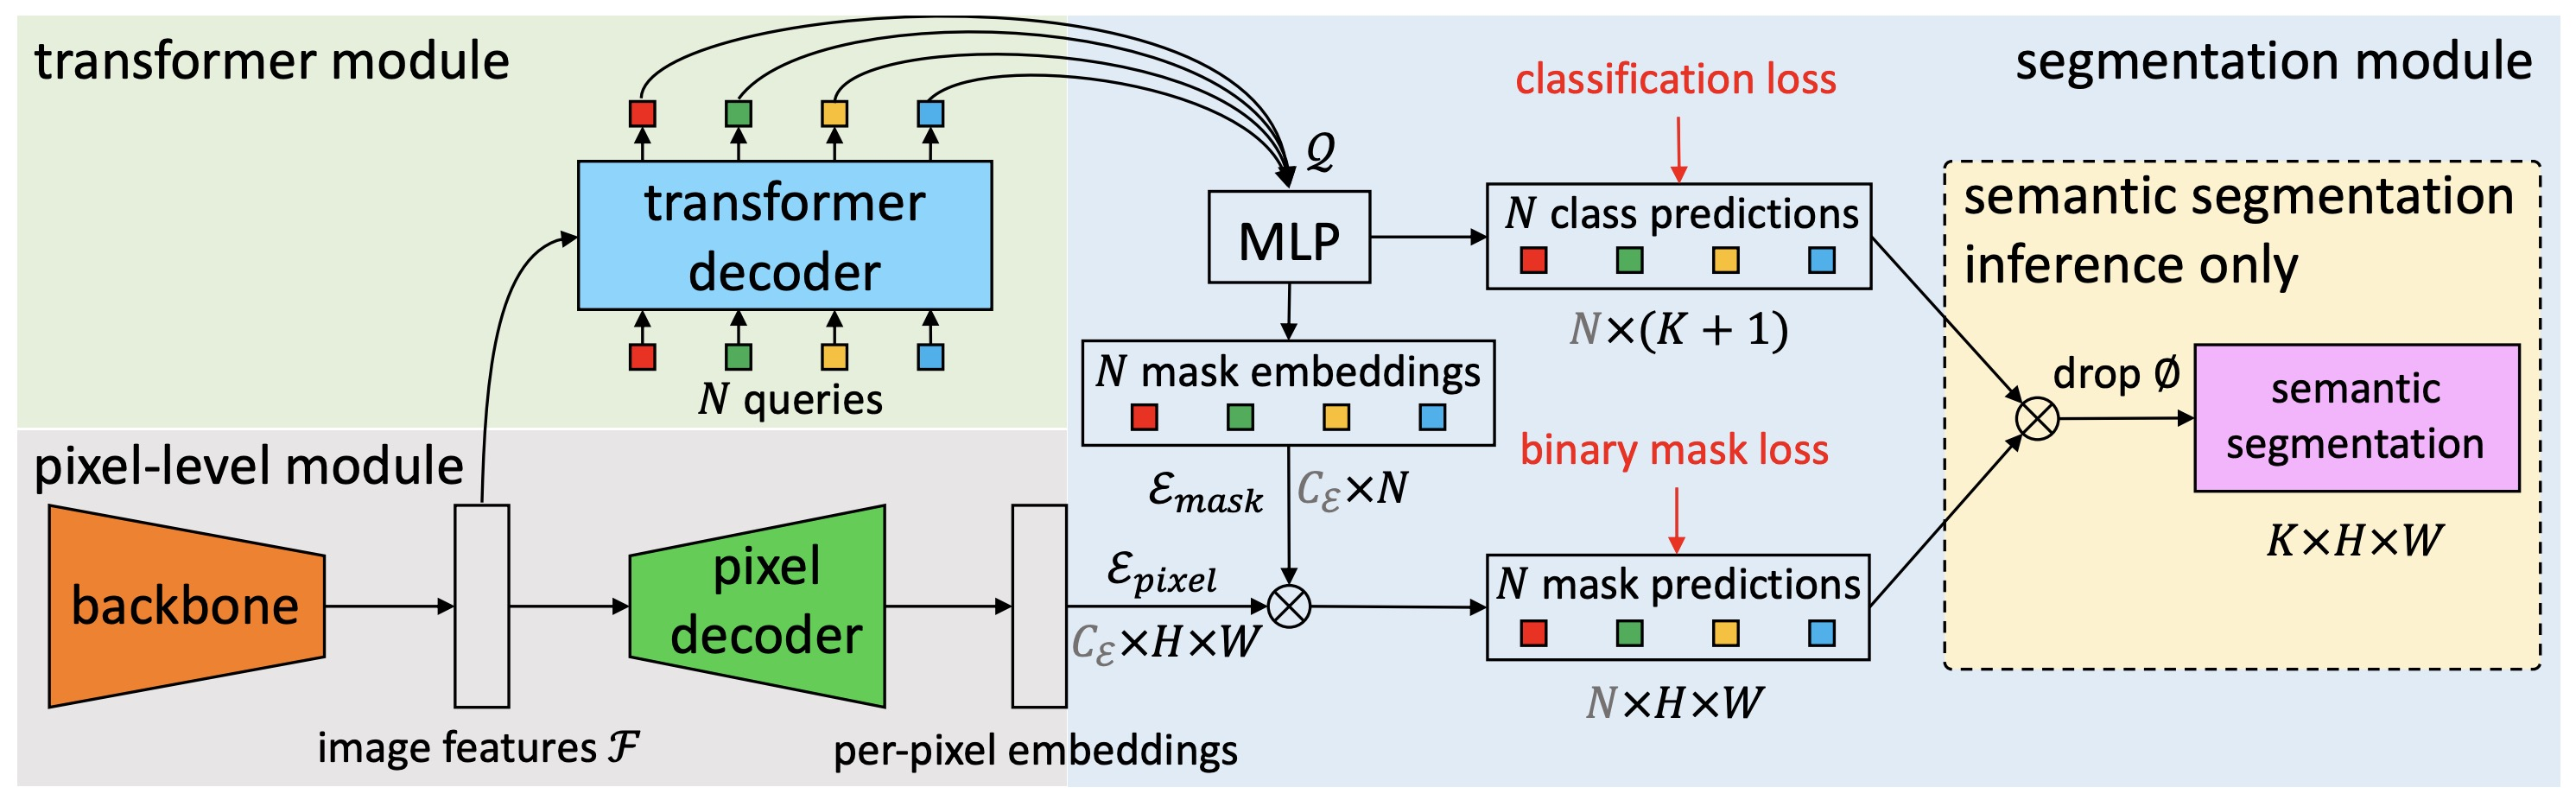
\includegraphics[width=0.62\textwidth]{figure/maskformer-architecture.jpg}\\
  \citebutton{Source: Cheng et al., 2021}{https://arxiv.org/abs/2107.06278}
\end{figure}
\vspace{-0.2cm}
{\small
\begin{itemize}
  \item \textbf{Pixel-level module}: a backbone extracts image features; a pixel decoder generates per-pixel embeddings.
  \item \textbf{Transformer module}: a standard Transformer decoder computes per-segment embeddings from image features and learnable queries.
  \item \textbf{Segmentation module}: class predictions (linear classifier) and mask embeddings (MLP) per segment; mask embeddings combined with per-pixel embeddings give a binary mask per segment.
\end{itemize}
}
\end{frame}

\begin{frame}{MaskFormer: Training and Fine-Tuning}
\small% fit16:9
\begin{itemize}
  \item MaskFormer predicts segmentation masks for each class present in an image, unifying semantic and instance segmentation in one architecture.
  \item Trained with a binary mask loss --- the same one as DETR --- plus a cross-entropy classification loss per predicted segment.
  \item \textbf{Panoptic segmentation}: label every pixel with its category \textit{and} identify distinct objects within those categories (semantic + instance). MaskFormer's output contains multiple instances of the same class, each with its own mask.
  \item Transformer-based segmentation models are data-hungry and hard to train from scratch, so transfer learning is common: typically the backbone, the pixel decoder and the Transformer decoder are frozen, and the rest is fine-tuned for new class predictions and masks.
\end{itemize}
\end{frame}

%%%%%%%%%%%%%%%%%%%%%%%%%%%%%%%%%%%%%%%%%%%%%%%%%%%%%%%%%%%%%%%%%%
\section{Knowledge Distillation with Vision Transformers}
% Source: HF CV course, unit3/vision-transformers/knowledge-distillation
%%%%%%%%%%%%%%%%%%%%%%%%%%%%%%%%%%%%%%%%%%%%%%%%%%%%%%%%%%%%%%%%%%

\begin{frame}{Knowledge Distillation: Intuition}
\begin{itemize}
  \item Instead of training a model on labels, \textbf{knowledge distillation} arrives at a much smaller model that performs comparably to a larger one --- and is much faster. It is the method behind DistilBERT and DistilGPT.
\end{itemize}
\begin{figure}
  \centering
  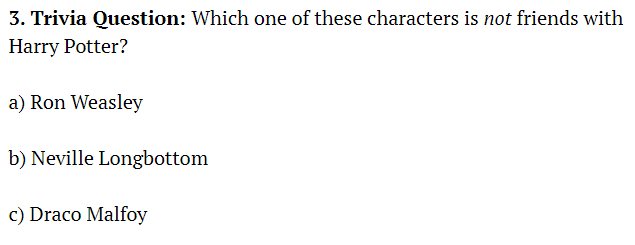
\includegraphics[width=0.45\textwidth]{figure/kd-question.png}
\end{figure}
\begin{itemize}
  \item Being told \enquote{the answer is Draco Malfoy} teaches you little about the characters' relationships to Harry Potter.
  \item \enquote{I am very confident it is \textit{not} Ron, somewhat confident it is not Neville, and very confident it \textit{is} Draco} carries much more information. This is the information passed to the student model.
\end{itemize}
\end{frame}

\begin{frame}{Distilling the Knowledge in a Neural Network}
\small% fit16:9
\begin{itemize}
  \item Introduced by Hinton et al.\ \citebutton{Hinton et al., 2015}{https://arxiv.org/abs/1503.02531}, inspired by insects: just as insects move from larval to adult forms optimized for different tasks, a cumbersome large model good at extracting structure from data can distill its knowledge into a smaller model for deployment.
  \item The teacher's predicted logits pass information to the student via a \textbf{distillation loss}, which encourages the student's output distribution to approximate the teacher's:
  $$L_{\text{distillation}} = \mathrm{KL}\big(\sigma(z_t; T=t),\, \sigma(z_s; T=t)\big)$$
  with teacher logits $z_t$, student logits $z_s$, softmax $\sigma$ at temperature $T$, and the Kullback-Leibler divergence KL.
  \item The student's overall loss: distillation loss + standard cross-entropy loss on the ground-truth labels.
\end{itemize}
\end{frame}

\begin{frame}{Distillation for Edge Devices}
\begin{itemize}
  \item Deploying a large model (e.g.\ 1\,GB, 1\,s latency) is impractical for real-time applications on edge devices. Distillation can reduce parameters by over 90\% with minimal performance degradation.
  \item \textbf{Consequences (good and bad):}
  \begin{enumerate}
    \item \textbf{Entropy gain}: which is harder to remember, \texttt{[0, 1, 0, 0]} or \texttt{[0.2, 0.5, 0.2, 0.1]}? The second contains more information. A distilled student's outputs have higher entropy than its teacher's: even when correct, they are more \enquote{chaotic}, since the teacher's extra parameters help it discern between classes.
  \end{enumerate}
\end{itemize}
\end{frame}

\begin{frame}{Distillation for Edge Devices (2)}
\begin{itemize}
  \item \textbf{Consequences (continued):}
  \begin{enumerate}
    \setcounter{enumi}{1}
    \item \textbf{Coherent gradient updates}: a misclassified ambiguous sample causes an aggressive update; the teacher's soft targets make updates more stable and coherent.
    \item \textbf{Training on unlabeled data}: the teacher can produce pseudo-labels for unlabeled samples.
    \item \textbf{A shift in perspective}: instead of approximating the unknown function $F$ from scarce data, approximate a well-trained teacher $F$ with a smaller model $f$.
  \end{enumerate}
\end{itemize}
\end{frame}

%%%%%%%%%%%%%%%%%%%%%%%%%%%%%%%%%%%%%%%%%%%%%%%%%%%%%%%%%%%%%%%%%%
\section{Introduction to Vision Language Models}
% Source: HF CV course, unit4/multimodal-models/vlm-intro
%%%%%%%%%%%%%%%%%%%%%%%%%%%%%%%%%%%%%%%%%%%%%%%%%%%%%%%%%%%%%%%%%%

\begin{frame}{Our World Is Multimodal}
\begin{itemize}
  \item Humans explore the world through diverse senses: sight, sound, touch, scent. Machine learning seeks models that process and integrate data across multiple \textbf{modalities}.
  \item Two key challenges:
  \begin{itemize}
    \item \textbf{Representation}: effectively summarizing multimodal data, capturing the connections among individual modality elements.
    \item \textbf{Alignment}: identifying connections and interactions across all elements.
  \end{itemize}
  \item Inherent difficulties: one modality may dominate the others; additional modalities can introduce noise; full coverage over all modalities is not guaranteed; modalities can have complicated relationships.
  \item This chapter: the fusion of vision and language --- \textbf{Vision Language Models (VLMs)}.
\end{itemize}
\end{frame}

\begin{frame}{From Training from Scratch to Pre-Training}
\small% fit16:9
\begin{itemize}
  \item Generating text from images (captioning, visual question answering) has been studied for years.
  \item A shift from training from scratch to the paradigm first proposed in ULMFiT \citebutton{Howard and Ruder, 2018}{https://aclanthology.org/P18-1031.pdf}:
  \begin{itemize}
    \item pre-train the model with extensive training data,
    \item fine-tune it with task-specific data,
    \item use it for downstream tasks such as classification.
  \end{itemize}
  \item VLMs extend this paradigm to images. In 2021, OpenAI's \textbf{CLIP} used an image-text \textbf{contrastive} objective: paired images and texts are brought close in the embedding space, all others pushed apart.
  \item This captures rich vision-language correspondence, enabling \textbf{zero-shot} predictions by matching embeddings of any image and text. CLIP outperformed ImageNet models on out-of-distribution tasks.
\end{itemize}
\end{frame}

\begin{frame}{VLM Mechanism}
\begin{itemize}
  \item Given image-text pairs: extract features with a text encoder and an image encoder (CNN- or Transformer-based), then learn the vision-language correlation with a pre-training objective:
  \begin{itemize}
    \item \textbf{contrastive}: pull paired samples close, push others far away in the embedding space;
    \item \textbf{generative}: learn semantic features by generating image/text data;
    \item \textbf{alignment}: global image-text matching or local region-word matching.
  \end{itemize}
  \item With the learned correlation, VLMs are evaluated zero-shot by matching embeddings of any given images and texts.
\end{itemize}
\begin{figure}
  \centering
  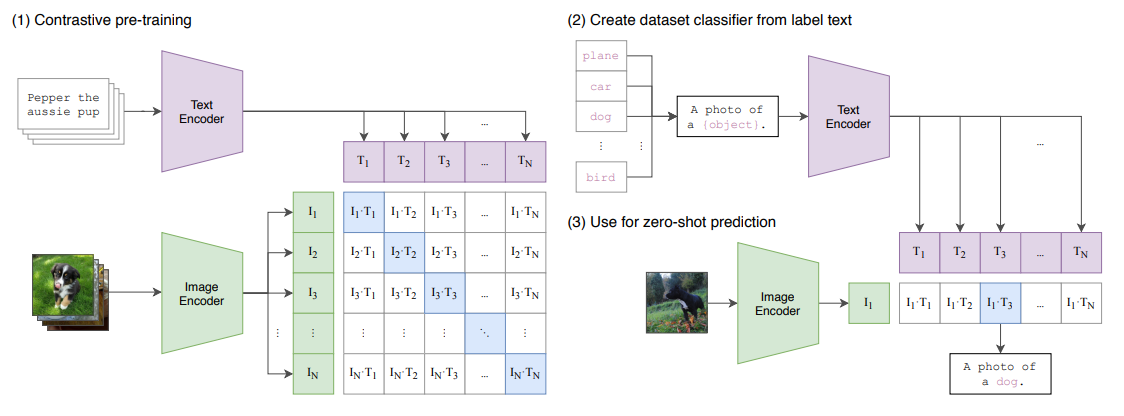
\includegraphics[width=0.27\textwidth]{figure/vlm-clip-mechanism.png}\\
  \citebutton{Source: Radford et al., 2021}{https://arxiv.org/abs/2103.00020}
\end{figure}
\end{frame}

\begin{frame}{VLM Strategies}
\small% fit16:9
Grouping VLMs by how they combine the two modes of learning:
\begin{itemize}
  \item \textbf{Images as tokens}: divide images into patches, treat each patch as a \enquote{token}, and train on joint sequences of text and image tokens (VisualBERT, SimVLM).
  \item \textbf{Image embeddings as a prefix} for a \textit{frozen} pre-trained language model: learn an image embedding space compatible with the language model's, without changing its parameters (Frozen, ClipCap).
  \item \textbf{Cross-attention}: a specially designed cross-attention mechanism fuses visual information into the layers of the language model (VisualGPT).
  \item \textbf{No training}: combine vision and language models via guided decoding of the next token (MAGiC).
\end{itemize}
\vspace{0.2cm}
Research focus: collecting large-scale informative image-text data, designing effective models for big data, and new pre-training objectives.
\end{frame}

\begin{frame}{Common VLM Datasets}
\begin{itemize}
  \item \textbf{MSCOCO}: 328K images, each paired with 5 independent captions.
  \item \textbf{NoCaps}: measures generalization to unseen classes and concepts (in-domain, near-domain, out-of-domain).
  \item \textbf{Conceptual Captions}: 3 million image-caption pairs, mined from the web and post-processed.
  \item \textbf{ALIGN}: a noisy dataset of over one billion image alt-text pairs, without expensive filtering or post-processing.
  \item \textbf{LAION}: image-text pairs extracted from Common Crawl (web pages crawled 2014--2021); used to train Stable Diffusion.
\end{itemize}
\end{frame}

\begin{frame}{Downstream Tasks and Evaluation}
\begin{itemize}
  \item Downstream tasks: image classification, object detection, semantic segmentation, image-text retrieval, action recognition.
  \item \textbf{Zero-shot prediction} (most common): apply the pre-trained VLM directly, without task-specific fine-tuning.
  \item \textbf{Linear probing}: freeze the VLM and train a linear classifier on its embeddings, measuring the quality of the representation.
  \item Harder datasets probe generalization: \textbf{Hateful Memes} adds difficult \enquote{benign confounders}; \textbf{Winoground} tests whether models truly grasp compositional relationships.
\end{itemize}
\begin{figure}
  \centering
  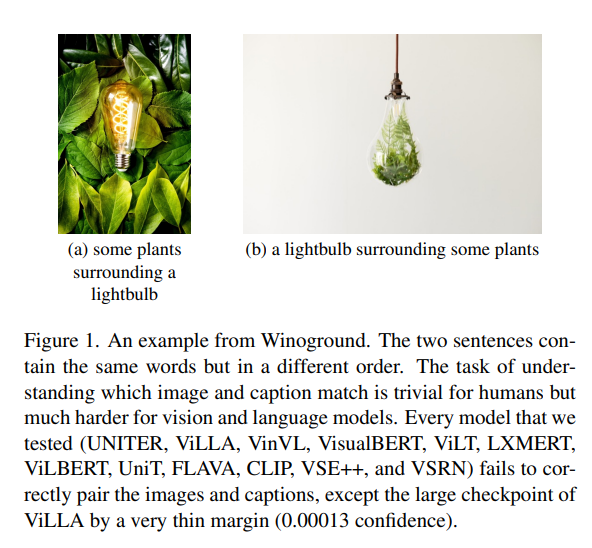
\includegraphics[width=0.20\textwidth]{figure/winoground.png}\\
  \citebutton{Source: Thrush et al., 2022}{https://arxiv.org/abs/2204.03162}
\end{figure}
\end{frame}

%%%%%%%%%%%%%%%%%%%%%%%%%%%%%%%%%%%%%%%%%%%%%%%%%%%%%%%%%%%%%%%%%%
\section{CLIP and Relatives}
% Source: HF CV course, unit4/multimodal-models/clip-and-relatives/Introduction
%%%%%%%%%%%%%%%%%%%%%%%%%%%%%%%%%%%%%%%%%%%%%%%%%%%%%%%%%%%%%%%%%%

\begin{frame}{Before and After CLIP}
\footnotesize% fit16:9

\textbf{Pre-CLIP:}
\begin{itemize}
  \item \textit{Multimodal Deep Learning} (Ngiam et al., 2011): deep learning for multimodal inputs.
  \item \textit{Deep Visual-Semantic Alignments} (Karpathy \& Fei-Fei, 2015): aligning text with specific image regions.
  \item \textit{Show and Tell} (Vinyals et al., 2015): CNNs and RNNs combined to turn images into descriptive language.
\end{itemize}
\textbf{Post-CLIP:}
\begin{itemize}
  \item \textbf{CLIP}: learns from a vast array of internet image-text pairs; zero-shot learning.
  \item \textbf{GroupViT}: segmentation and semantic understanding combined with language.
  \item \textbf{BLIP}: bidirectional learning between vision and language; generating text from images.
  \item \textbf{OWL-ViT}: object-centric representations, understanding objects in images in context with text.
\end{itemize}
\end{frame}

%%%%%%%%%%%%%%%%%%%%%%%%%%%%%%%%%%%%%%%%%%%%%%%%%%%%%%%%%%%%%%%%%%
\section{Losses}
% Source: HF CV course, unit4/multimodal-models/clip-and-relatives/losses
%%%%%%%%%%%%%%%%%%%%%%%%%%%%%%%%%%%%%%%%%%%%%%%%%%%%%%%%%%%%%%%%%%

\begin{frame}{Contrastive Learning}
\begin{itemize}
  \item \textbf{Contrastive learning}: an unsupervised method for representation learning.
  \item Objective: a representation in which similar items are positioned close together and dissimilar items are clearly separated.
  \item Example: keep the representations of dogs close to other dogs, but far from cats.
\end{itemize}
\begin{figure}
  \centering
  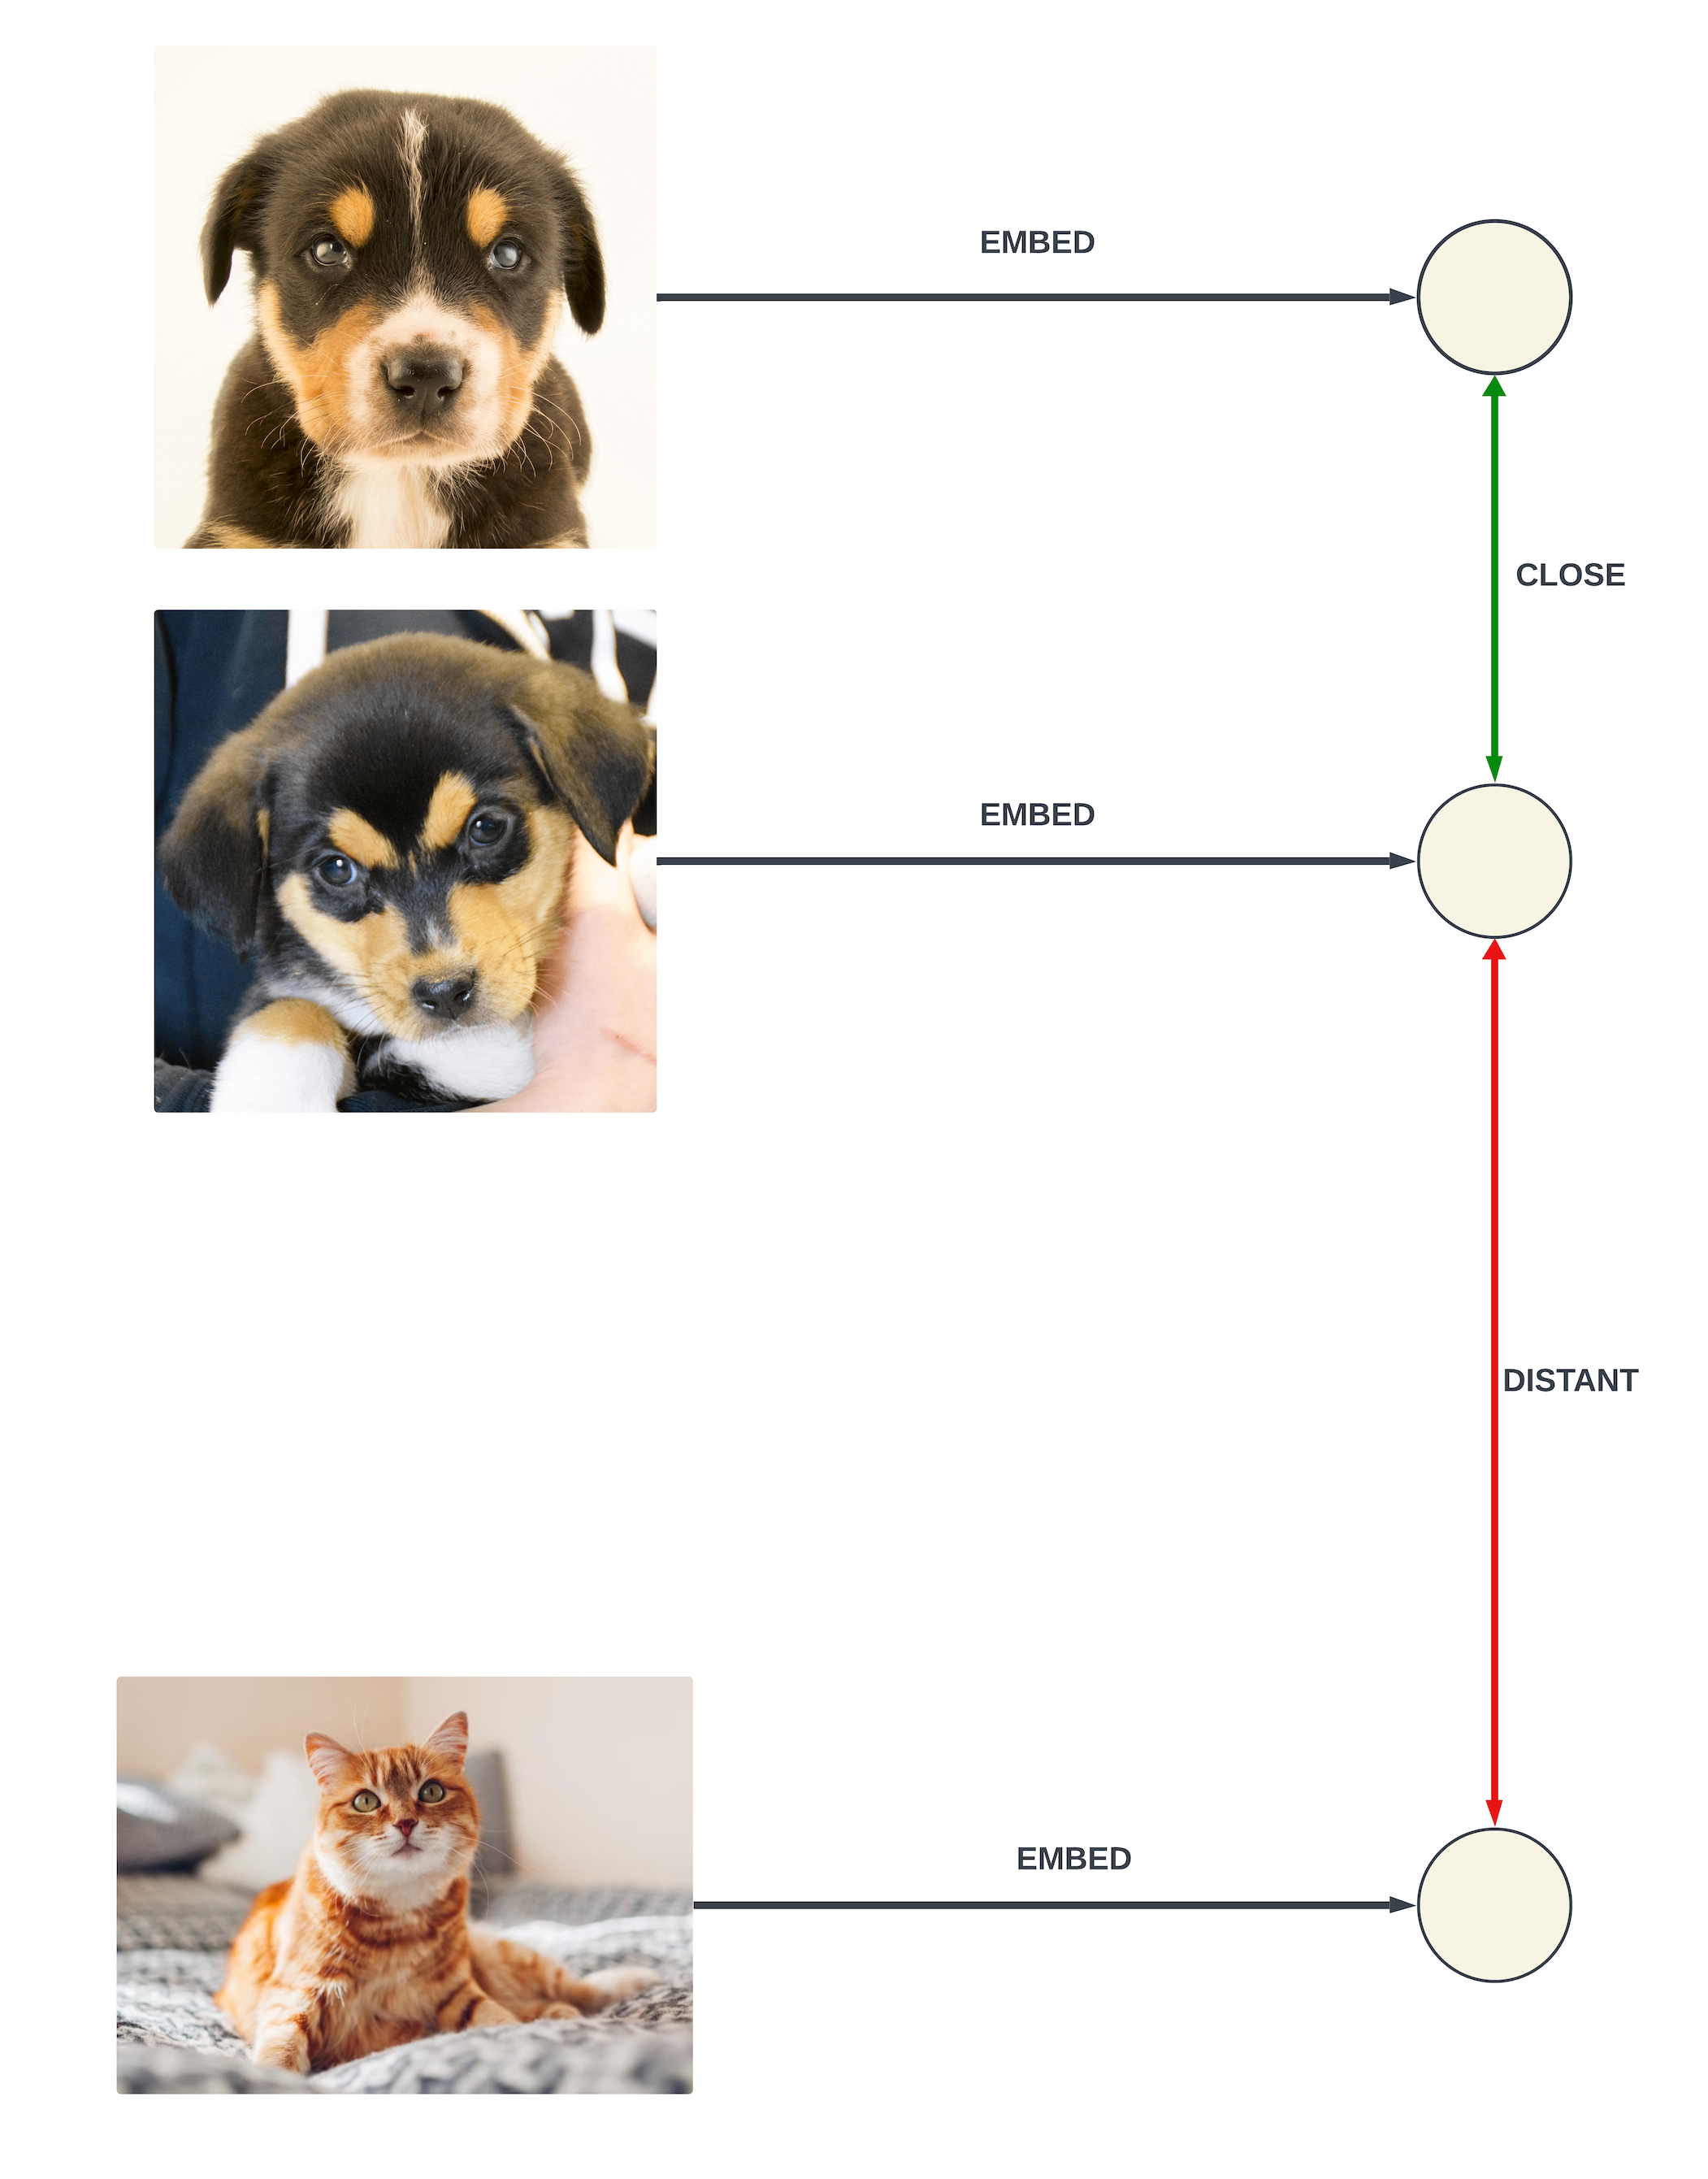
\includegraphics[height=3.4cm]{figure/contrastive-learning.png}
\end{figure}
\end{frame}

\begin{frame}{Contrastive Loss}
\begin{itemize}
  \item One of the first training objectives for contrastive learning. Input: a pair of samples, similar or dissimilar. Goal: map similar samples close in the embedding space, push dissimilar ones apart.
  \item For samples $x_i, x_j$ with classes $y_i, y_j$:
  $$L = \mathbb{1}[y_i = y_j]\,\|x_i - x_j\|^2 + \mathbb{1}[y_i \neq y_j]\,\max(0, \epsilon - \|x_i - x_j\|^2)$$
  \item If the samples are similar ($y_i = y_j$): minimize their squared Euclidean distance --- make them closer.
  \item If they are dissimilar ($y_i \neq y_j$): minimizing $\max(0, \epsilon - \|x_i - x_j\|^2)$ means maximizing their distance, up to a margin $\epsilon$.
\end{itemize}
\end{frame}

%%%%%%%%%%%%%%%%%%%%%%%%%%%%%%%%%%%%%%%%%%%%%%%%%%%%%%%%%%%%%%%%%%
\section{Contrastive Language-Image Pre-training (CLIP)}
% Source: HF CV course, unit4/multimodal-models/clip-and-relatives/clip
%%%%%%%%%%%%%%%%%%%%%%%%%%%%%%%%%%%%%%%%%%%%%%%%%%%%%%%%%%%%%%%%%%

\begin{frame}{CLIP}
\begin{itemize}
  \item CLIP \citebutton{Radford et al., 2021}{https://arxiv.org/abs/2103.00020} grasps visual concepts through \textbf{natural language supervision}: a text encoder and an image encoder are trained jointly on matching captions with their images.
  \item It adapts to a variety of visual classification benchmarks by simply receiving the \textit{names} of the visual categories to be recognized --- \enquote{zero-shot} capabilities akin to those of GPT-2 and GPT-3.
\end{itemize}
\end{frame}

\begin{frame}{Contrastive Pre-Training}
\begin{figure}
  \centering
  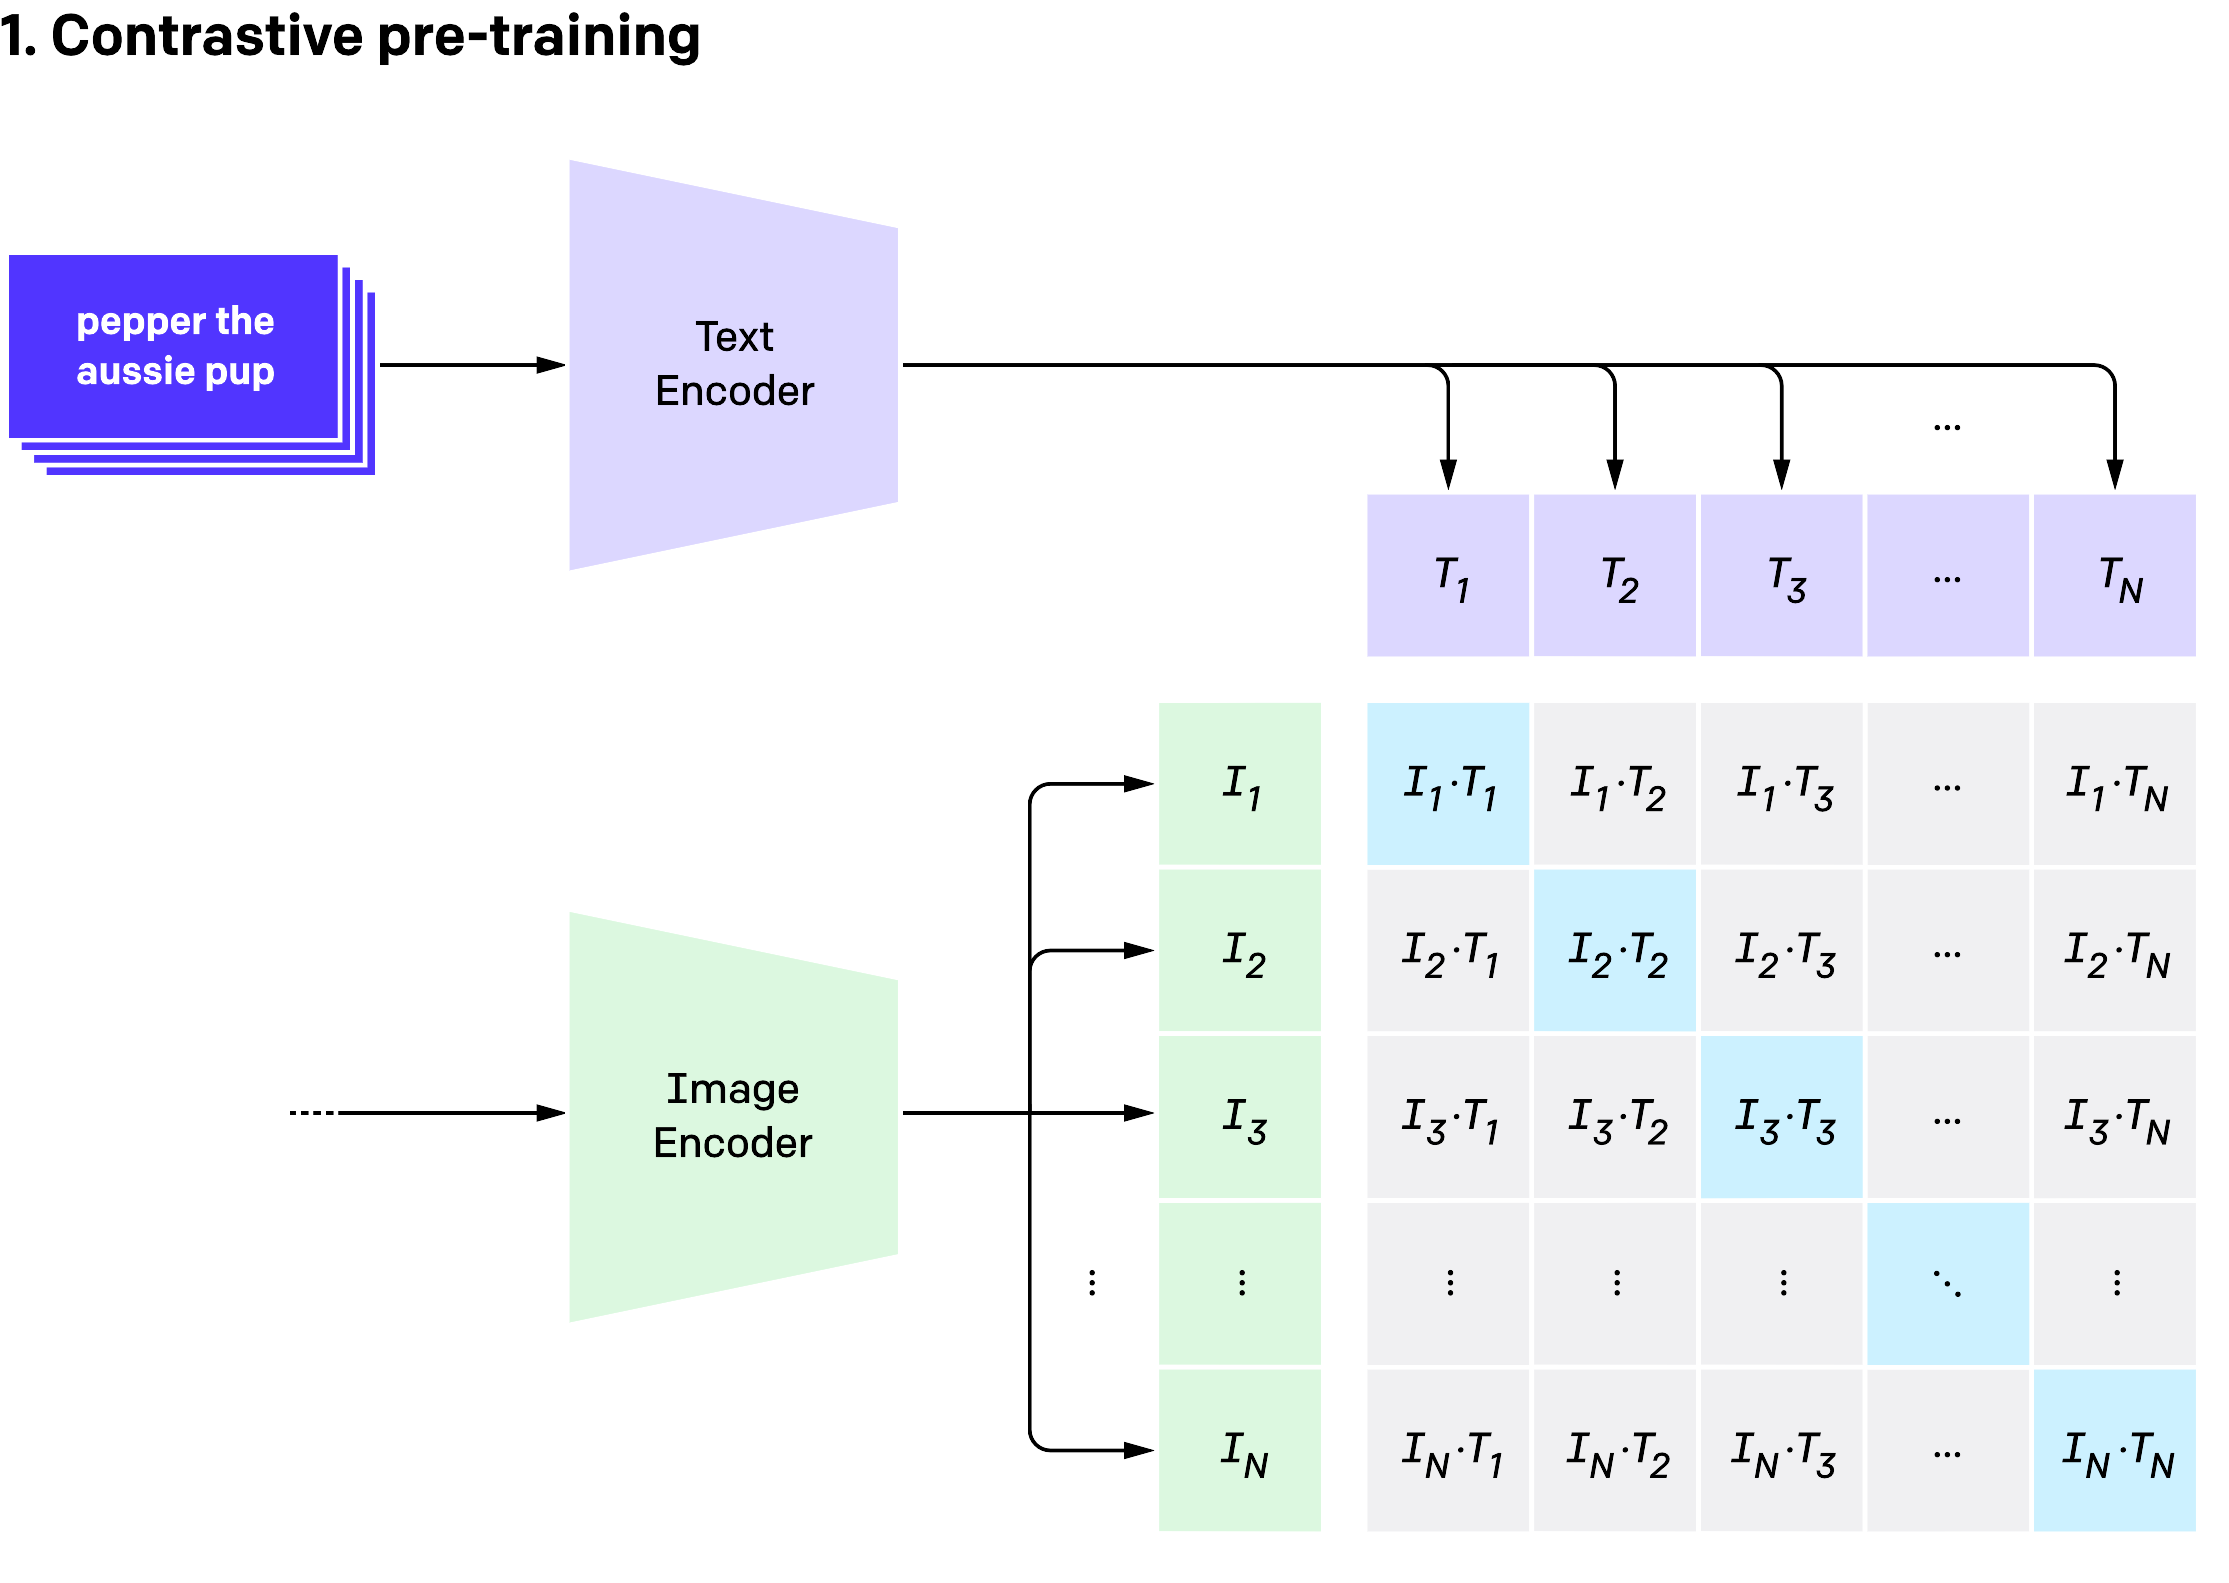
\includegraphics[height=2.80cm]{figure/clip-overview.png}\\
  \citebutton{Source: OpenAI}{https://openai.com/research/clip}
\end{figure}
\vspace{-0.3cm}
{\small
\begin{itemize}
  \item Given a batch of image-text pairs, compute the cosine similarity matrix between all possible (image, text) candidates.
  \item Maximize the similarity of correct pairs (blue diagonal), minimize it for incorrect pairs, via a \textbf{symmetric cross-entropy loss} over the similarity scores.
  \item In simple terms: each image should be most similar to its own caption, and each caption to its own image.
\end{itemize}
}
\end{frame}

\begin{frame}{CLIP: Encoders, Use Cases, Limitations}
\begin{itemize}
  \item \textbf{Independent encoders} for images and text: e.g.\ a Vision Transformer or a ResNet as image encoder. Switching an encoder requires retraining, as the embedding distribution changes.
  \item \textbf{Use cases}: zero-shot image classification, similarity search, conditioning diffusion models.
  \item \textbf{Limitations}:
  \begin{itemize}
    \item Unlikely to outperform a specialized, fine-tuned model; generalization is limited for data not encountered during training.
    \item Effectiveness and biases depend on the choice of categories: on the FairFace dataset, gender accuracy was over 96\%, racial accuracy around 93\%.
  \end{itemize}
\end{itemize}
\end{frame}

\begin{frame}[fragile]{CLIP: Zero-Shot Classification in Practice}
\scriptsize
\begin{verbatim}
from transformers import CLIPProcessor, CLIPModel

model = CLIPModel.from_pretrained("openai/clip-vit-base-patch32")
processor = CLIPProcessor.from_pretrained("openai/clip-vit-base-patch32")

inputs = processor(text=["a photo of a cat", "a photo of a dog"],
                   images=image, return_tensors="pt", padding=True)
outputs = model(**inputs)
probs = outputs.logits_per_image.softmax(dim=1)
\end{verbatim}
\normalsize
\begin{itemize}
  \item Zero-shot classification of a photo of cats between \texttt{dog} and \texttt{cat}: the class names become text prompts, and the image is matched against them.
  \item Result: \enquote{a photo of a cat} 99.49\%, \enquote{a photo of a dog} 0.51\%.
\end{itemize}
\end{frame}

%%%%%%%%%%%%%%%%%%%%%%%%%%%%%%%%%%%%%%%%%%%%%%%%%%%%%%%%%%%%%%%%%%
\section{Multimodal Text Generation (BLIP)}
% Source: HF CV course, unit4/multimodal-models/clip-and-relatives/blip
%%%%%%%%%%%%%%%%%%%%%%%%%%%%%%%%%%%%%%%%%%%%%%%%%%%%%%%%%%%%%%%%%%

\begin{frame}{BLIP: Bootstrapping Language-Image Pre-Training}
\begin{itemize}
  \item BLIP \citebutton{Li et al., 2022}{https://arxiv.org/abs/2201.12086} extends multimodal models to \textbf{text generation}.
  \item \textbf{CapFilt (caption and filtering)}: web-scraped image/alt-text pairs are noisy --- alt-texts often do not describe the image. One model filters out noisy pairs, another creates captions for images; both are first fine-tuned on a human-annotated dataset. Cleaning the data this way beat training on the raw web data.
  \item Takeaway: dataset \textbf{quality} matters, not just quantity.
  \item Successor: BLIP-2 \citebutton{Li et al., 2023}{https://arxiv.org/abs/2301.12597}, e.g.\ for visual question answering.
\end{itemize}
\end{frame}

\begin{frame}{BLIP: Architecture}
A vision encoder plus a \textbf{Multimodal mixture of Encoder-Decoder (MED)}:
\begin{itemize}
  \item \textbf{Vision Transformer}: a plain ViT with a {\tt [CLS]} token for the embedding.
  \item \textbf{Unimodal text encoder}: like BERT, with a {\tt [CLS]} token; trained with a contrastive loss like CLIP to align image and text representations.
  \item \textbf{Image-grounded text encoder}: {\tt [CLS]} replaced by an {\tt [Encode]} token; cross-attention layers combine image and text embeddings into a multimodal representation; a linear layer judges whether image and text match.
  \item \textbf{Image-grounded text decoder}: bidirectional self-attention replaced by \textbf{causal} self-attention; trained autoregressively with cross-entropy, for caption generation or visual question answering.
\end{itemize}
\end{frame}

%%%%%%%%%%%%%%%%%%%%%%%%%%%%%%%%%%%%%%%%%%%%%%%%%%%%%%%%%%%%%%%%%%
\section{Multimodal Object Detection (OWL-ViT)}
% Source: HF CV course, unit4/multimodal-models/clip-and-relatives/owl_vit
%%%%%%%%%%%%%%%%%%%%%%%%%%%%%%%%%%%%%%%%%%%%%%%%%%%%%%%%%%%%%%%%%%

\begin{frame}{OWL-ViT: Open-Vocabulary Object Detection}
\begin{itemize}
  \item Detectors like YOLO cannot detect objects outside their training datasets. OWL-ViT \citebutton{Minderer et al., 2022}{https://arxiv.org/abs/2205.06230} is akin to CLIP, but for object detection.
  \item \textbf{Pre-training}: like CLIP, a vision and a language encoder with a contrastive loss --- a shared representation space for images and text.
  \item \textbf{Fine-tuning for detection}: instead of CLIP's token pooling and final projection, each output token is linearly projected to a per-object image embedding used for classification; box coordinates come from the token representations via a small MLP.
\end{itemize}
\begin{figure}
  \centering
  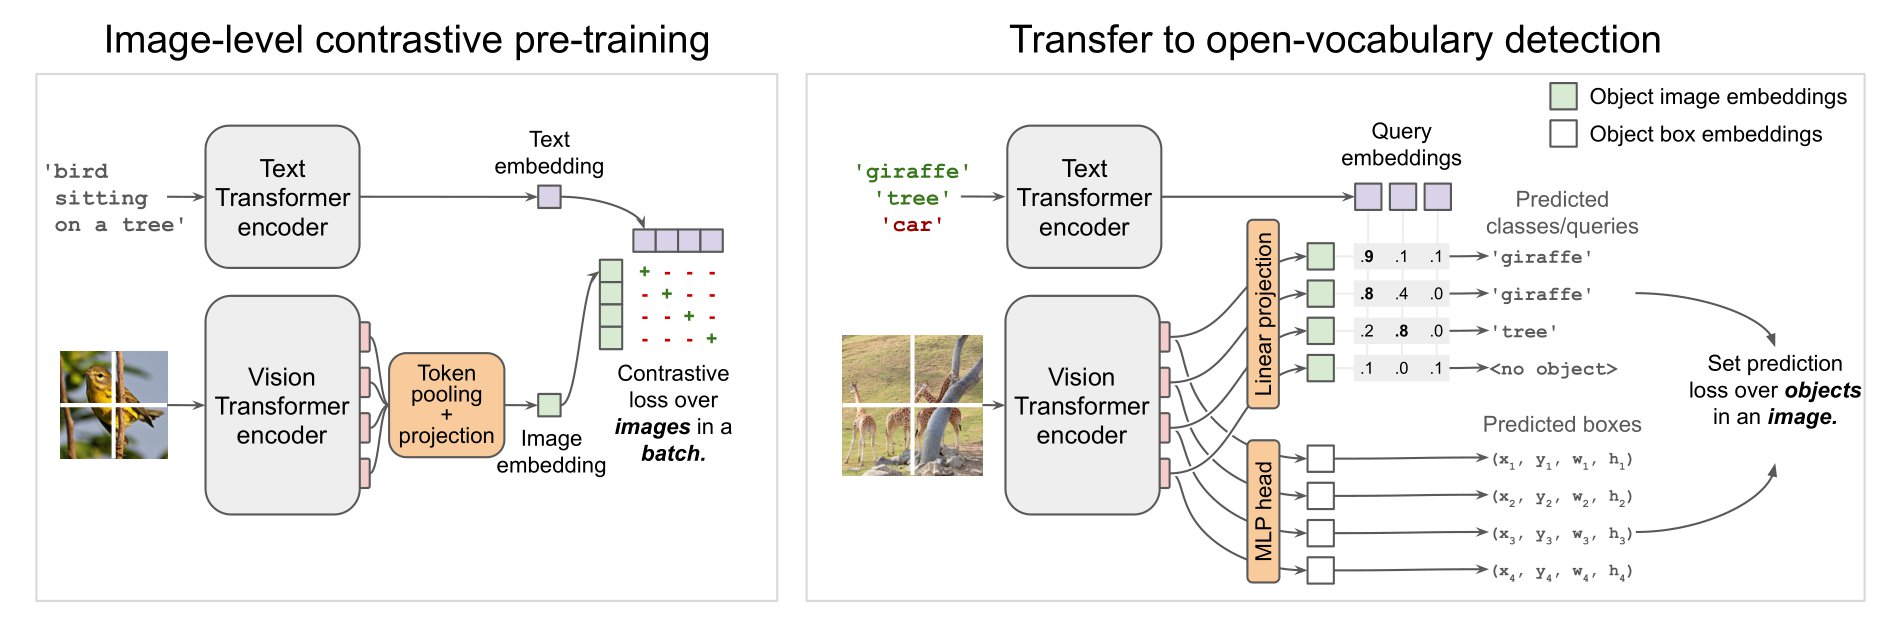
\includegraphics[width=0.14\textwidth]{figure/owlvit-architecture.jpg}\\
  \citebutton{Source: Minderer et al., 2022}{https://arxiv.org/abs/2205.06230}
\end{figure}
\end{frame}

\begin{frame}{OWL-ViT: Example}
\begin{itemize}
  \item Thanks to the shared embedding space, OWL-ViT identifies objects not present in its training data; both images and text can be used as queries.
  \item Example: text queries for objects likely in detection datasets (\enquote{cat}) and more abstract ones (\enquote{cat tail}) that most likely are not.
\end{itemize}
\begin{figure}
  \centering
  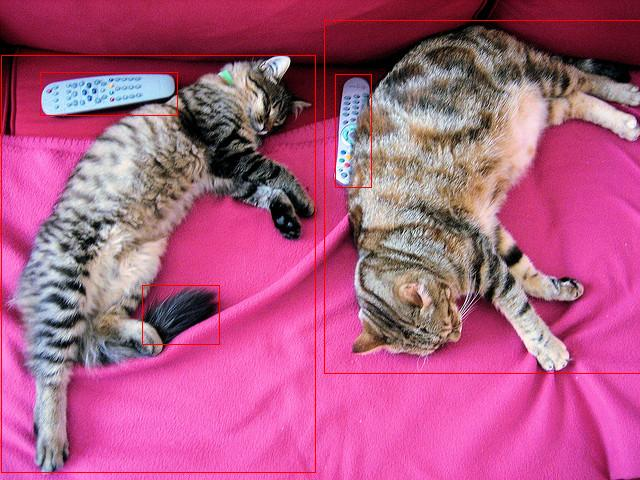
\includegraphics[height=3.6cm]{figure/owlvit-example.jpg}
\end{figure}
\end{frame}

%%%%%%%%%%%%%%%%%%%%%%%%%%%%%%%%%%%%%%%%%%%%%%%%%%%%%%%%%%%%%%%%%%
\section{Transformers in Video Processing}
% Source: HF CV course, unit7/video-processing/transformers-based-models
%%%%%%%%%%%%%%%%%%%%%%%%%%%%%%%%%%%%%%%%%%%%%%%%%%%%%%%%%%%%%%%%%%

\begin{frame}{Recap: ViT}
\begin{figure}
  \centering
  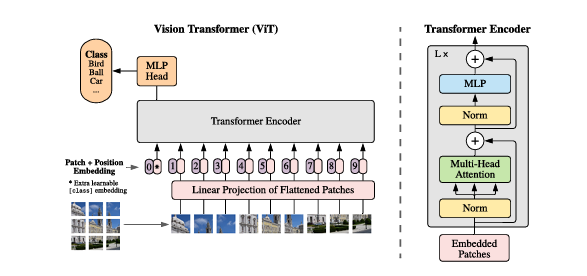
\includegraphics[width=0.5\textwidth]{figure/vit-architecture.png}\\
  \citebutton{Source: Dosovitskiy et al., 2020}{https://arxiv.org/abs/2010.11929}
\end{figure}
\begin{itemize}
  \item Images are divided into small patches; each patch is an input to a Transformer, replacing CNNs.
  \item Each patch is linearly mapped, and positional embeddings are added so the Transformer can recognize the order of the patches.
  \item Pre-trained on large-scale datasets and fine-tuned for downstream vision tasks.
\end{itemize}
\end{frame}

\begin{frame}{ViT: Performance and Limitation}
\begin{figure}
  \centering
  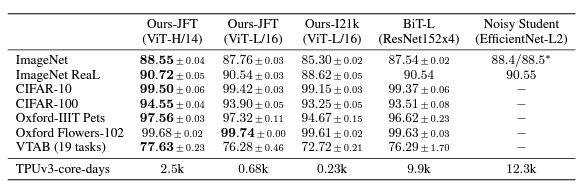
\includegraphics[width=0.75\textwidth]{figure/vit-performance.jpg}\\
  \citebutton{Source: Dosovitskiy et al., 2020}{https://arxiv.org/abs/2010.11929}
\end{figure}
\begin{itemize}
  \item ViT outperformed other state-of-the-art models, but training it required 2{,}500 TPU-v3 days. At roughly \$2 per TPU-v3 core-hour, one training run costs about $2 \times 24 \times 2500 = $ \$120{,}000.
\end{itemize}
\end{frame}

\begin{frame}{Video Vision Transformer (ViViT)}
\begin{itemize}
  \item ViViT \citebutton{Arnab et al., 2021}{https://arxiv.org/abs/2103.15691} extends ViT to video classification. Key issues: train more quickly and efficiently, and handle \textbf{temporal} as well as spatial information.
  \item Extracts spatio-temporal tokens from the video and encodes them with Transformer layers; efficient variants factorise the spatial and temporal dimensions; pre-trained image models make training on comparatively small datasets possible.
\end{itemize}
\begin{figure}
  \centering
  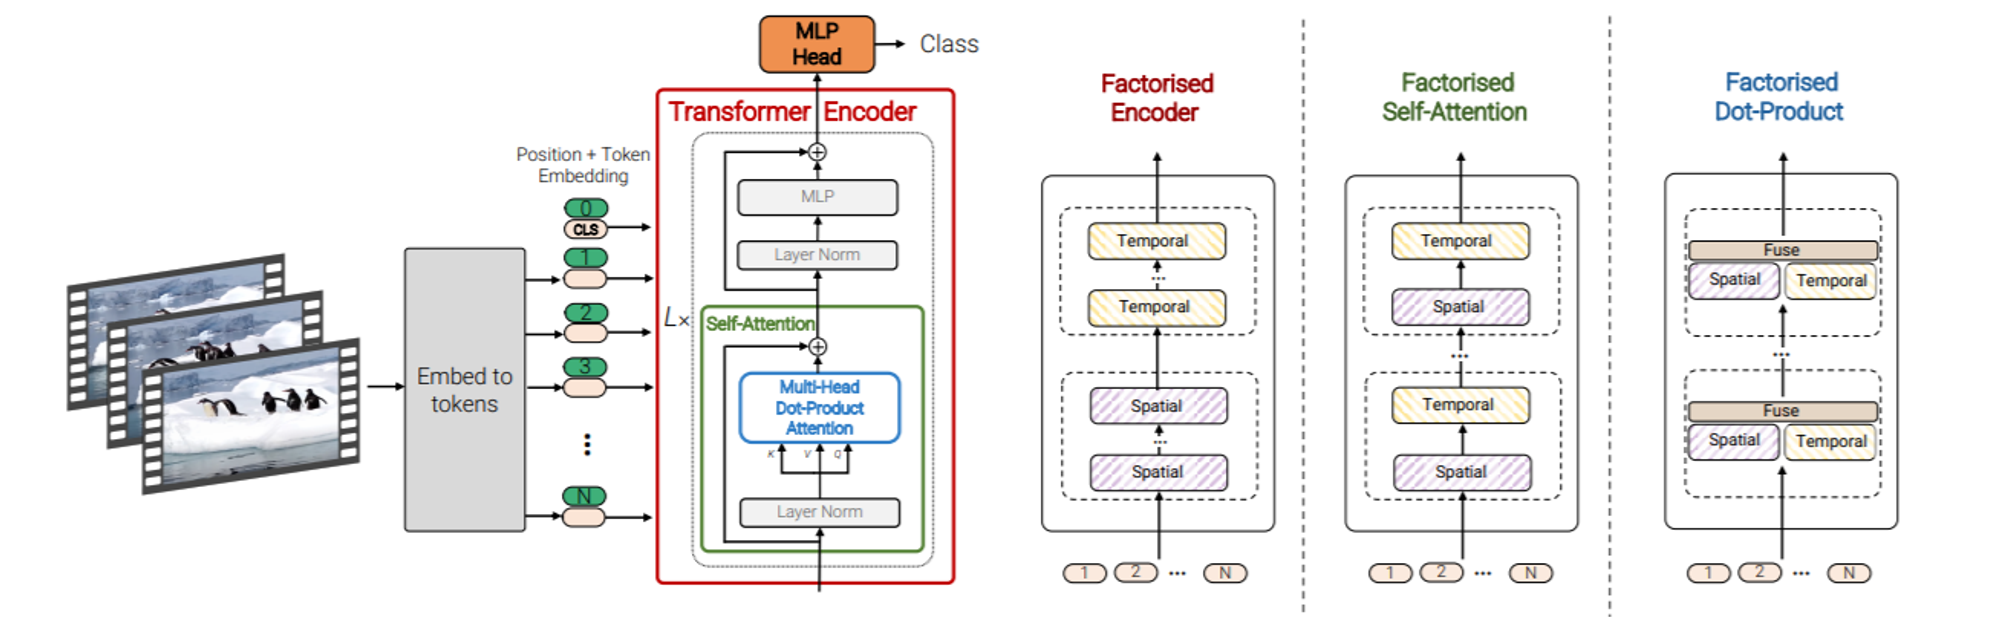
\includegraphics[width=0.72\textwidth]{figure/vivit-architecture.png}\\
  \citebutton{Source: Arnab et al., 2021}{https://arxiv.org/abs/2103.15691}
\end{figure}
\end{frame}

\begin{frame}{Embedding Video Clips}
\begin{itemize}
  \item Embeddings: dense vectors capturing meaningful features. For video, they must preserve \textbf{spatial} (what is in each frame) and \textbf{temporal} (how things change) information, while reducing dimensionality so processing stays feasible.
\end{itemize}
\begin{columns}
\begin{column}{0.48\textwidth}
\centering
\textbf{Uniform frame sampling}\\
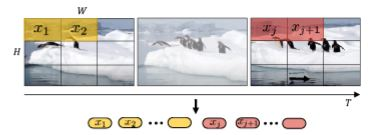
\includegraphics[width=0.8\textwidth]{figure/vivit-uniform-sampling.jpg}\\
{\footnotesize Sample frames uniformly over time, e.g.\ one in every 2 frames.}
\end{column}
\begin{column}{0.48\textwidth}
\centering
\textbf{Tubelet embedding}\\
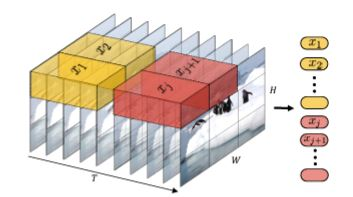
\includegraphics[width=0.8\textwidth]{figure/vivit-tubelet.jpg}\\
{\footnotesize Extract spatio-temporal \enquote{tubes} and project them linearly: fuses space and time already during tokenization.}
\end{column}
\end{columns}
\vspace{0.1cm}
{\footnotesize Figures: \citebutton{Arnab et al., 2021}{https://arxiv.org/abs/2103.15691}}
\end{frame}

\begin{frame}{ViViT Model 1: Spatio-Temporal Attention}
\begin{itemize}
  \item The natural extension of ViT: each of the $n_t$ frames is split into $n_w \times n_h$ patches, giving $n_t \times n_w \times n_h$ \textbf{spatio-temporal tokens}.
  \item All tokens go through the Transformer encoder together, so each token is contextualized with all others across space and time --- patterns in position, color and movement.
  \item Complexity: $\mathcal{O}(n_h^2\, n_w^2\, n_t^2)$.
  \item Attention over all spatio-temporal tokens is expensive; uniform frame sampling and tubelet embedding help reduce the cost.
\end{itemize}
\end{frame}

\begin{frame}{ViViT Model 2: Factorised Encoder}
\begin{figure}
  \centering
  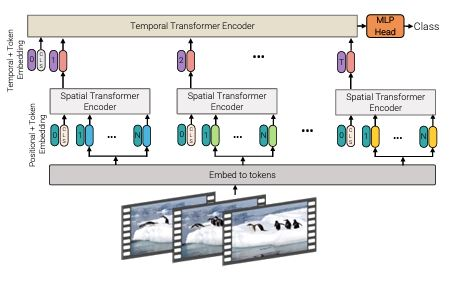
\includegraphics[height=2.9cm]{figure/vivit-model2.jpg}\\
  \citebutton{Source: Arnab et al., 2021}{https://arxiv.org/abs/2103.15691}
\end{figure}
\vspace{-0.3cm}
{\small
\begin{itemize}
  \item Model 1 contextualizes all patches simultaneously --- inefficient. Model 2 separates spatial and temporal encoders, sequentially:
  \begin{itemize}
    \item a \textbf{spatial} Transformer encoder (= ViT) contextualizes within each frame and encodes it into a single embedding;
    \item a \textbf{temporal} Transformer encoder then processes the frame embeddings.
  \end{itemize}
  \item Complexity: $\mathcal{O}(n_h^2\, n_w^2 + n_t^2)$.
\end{itemize}
}
\end{frame}

\begin{frame}{ViViT Models 3 and 4}
\begin{columns}
\begin{column}{0.48\textwidth}
\centering
\textbf{Model 3: Factorised Self-Attention}\\
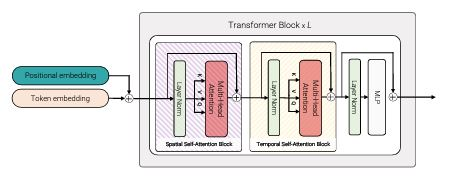
\includegraphics[width=0.85\textwidth]{figure/vivit-model3.jpg}\\
{\footnotesize First self-attention \textbf{spatially} (among tokens of the same time index), then \textbf{temporally} (among tokens of the same spatial index). No {\tt [CLS]} token, because of ambiguities.}
\end{column}
\begin{column}{0.48\textwidth}
\centering
\textbf{Model 4: Factorised Dot-Product Attention}\\
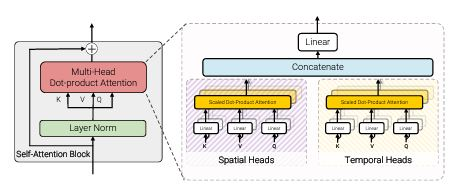
\includegraphics[width=0.85\textwidth]{figure/vivit-model4.jpg}\\
{\footnotesize Half of the attention heads use keys and values from the same spatial indices, the other half from the same temporal indices.}
\end{column}
\end{columns}
\vspace{0.1cm}
{\footnotesize Complexity of both: same as Model 2. Figures: \citebutton{Arnab et al., 2021}{https://arxiv.org/abs/2103.15691}}
\end{frame}

\begin{frame}{ViViT: Experiments and Discussion}
\begin{figure}
  \centering
  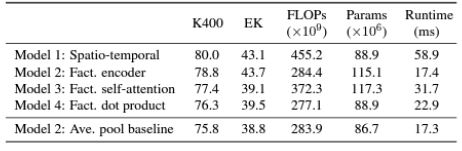
\includegraphics[width=0.55\textwidth]{figure/vivit-performance.jpg}\\
  \citebutton{Source: Arnab et al., 2021}{https://arxiv.org/abs/2103.15691}
\end{figure}
\begin{itemize}
  \item Model 1 achieves the best accuracy but needs the longest training; Model 2 gives relatively high accuracy with shorter training than Models 3 and 4 --- the most efficient overall.
  \item Like ViT, ViViT needs extremely large datasets, which rarely exist for video. Approach: first pre-train on a large image dataset with ViT to initialize the model.
\end{itemize}
\end{frame}

\begin{frame}{TimeSformer}
Concurrent work with ViViT \citebutton{Bertasius et al., 2021}{https://arxiv.org/abs/2102.05095}; five space-time self-attention schemes (blue: query patch):
\begin{figure}
  \centering
  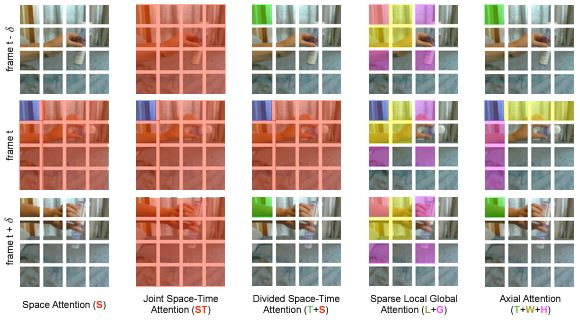
\includegraphics[height=1.88cm]{figure/timesformer.jpg}
\end{figure}
\vspace{-0.3cm}
{\small
\begin{itemize}
  \item \textbf{Space}: as in ViT, within one frame. \textbf{Joint space-time}: across frames, as ViViT Model 1.
  \item \textbf{Divided space-time}: first temporally (same position, other frames), then spatially --- similar to ViViT Model 3.
  \item \textbf{Sparse local global}: selectively combines local and global information. \textbf{Axial}: spatial and temporal dimensions separately along their axes.
  \item \textbf{Divided space-time attention} gives the best balance of parameter efficiency and accuracy (K400, SSv2).
\end{itemize}
}
\end{frame}

\begin{frame}{Conclusion: Video Transformers}
\begin{itemize}
  \item ViViT extended ViT to video with several models (factorised encoder, factorised self-attention, factorised dot-product attention), all aimed at managing the space-time dimensions efficiently.
  \item TimeSformer likewise evolved from ViT, using diverse attention mechanisms over space and time.
  \item Key takeaway: the focus is on reducing the significant computational cost of applying Transformers to video, enabling learning with fewer computational resources.
\end{itemize}
\end{frame}

%%%%%%%%%%%%%%%%%%%%%%%%%%%%%%%%%%%%%%%%%%%%%%%%%%%%%%%%%%%%%%%%%%
\section{License \& Attribution}
%%%%%%%%%%%%%%%%%%%%%%%%%%%%%%%%%%%%%%%%%%%%%%%%%%%%%%%%%%%%%%%%%%

\begin{frame}{License \& Attribution}
\begin{itemize}
\item \textbf{Single source.} All content follows the \textbf{Hugging Face Community Computer Vision Course} (\url{https://huggingface.co/learn/computer-vision-course}, repository \url{https://github.com/johko/computer-vision-course}, \copyright\ 2023 Johannes Kolbe and contributors) --- licensed \textbf{MIT}. Units 3 (\textit{Vision Transformers}), 4 (\textit{Multimodal Models}) and 7 (\textit{Video}), in the course's own order. The course is prose, not slides: frames condense its text into bullet points without adding content.
\item \textbf{Figures} are those the course uses, with the attribution the course gives: most are taken from the original papers (linked on each frame); the CLIP pre-training figure is from OpenAI; the MaskFormer and OWL-ViT figures come via the Hugging Face documentation.
\end{itemize}
\end{frame}

\endlecture
\end{document}
